\chapter{Results}
\section{Simulation of Capacitance values}
\subsection{Comparision of Capacitance in the simulation with a sphere geometry}

\begin{figure}[htbp]
	\centering
	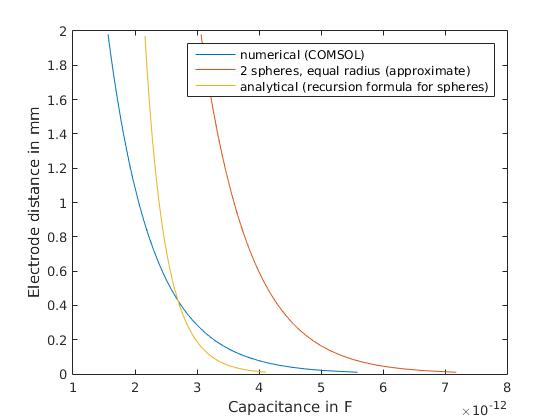
\includegraphics[scale=0.3]{figures/Capacitance_comparision.jpg}		
	\caption[Kurze Abbildungsbeschreibung]{Electron drift currents in Ar at 30 Td and in CO$_2$ at 65 Td, the latter was divided by 10 and shifted by 0.2 $\mu$s. Dotted lines are averages of measured waveforms, solid lines are fits of Eq. XX. $T$ marks the electron transit time, and the markers $T_1$ to $T_3$ are explained in section.} %\ref{sec.analysecurrent}
	\label{fig.waveforms}
\end{figure}

\section{Complex effective permittivity}
\subsection{}

\section{Performance of integrator}

\section{Dielectric Spectroscopy}

\begin{figure}[htbp]
\end{figure}
